%\section{Если из А следует B и B приятно, то A -- истина.}

В \textbf{третьей главе} построены две динамические модели экипажа на плоскости с трением. В одной модели используется сухое трение Амонтона -- Кулона, регуляризованное в окрестности нуля по скоростям участком линейной функции насыщения с достаточно большим угловым коэффициентом. В другой модели используется вязкое трение. Рассматриваются две конструкции колеса: обыкновенное омни-колесо, оси роликов которого лежат в плоскости, содержащей диск колеса, и колесо \textit{mecanum}, оси роликов которого находятся под углом к плоскости диска колеса. Особое внимание уделяется вопросу моделирования связи в контакте ролика и горизонтальной плоскости, отслеживанию точки контакта ролика и опорной плоскости, а также алгоритмической реализации процесса переключения контакта от ролика к ролику при качении омни-колеса. Динамические модели построены в формализме объектно-ориентированного моделирования на языке \texttt{Modelica}. Выполнена верификация динамической модели с использованием безынерционной модели.

%\chapter{Динамика экипажа на омни-колесах с трением}
%

В начале главы описан формализм для описания динамики систем тел, использованный для построения моделей экипажа. Положение каждого твердого тела задается радиусом-вектором центра масс тела $\vec{r}$ в неподвижной системе отсчета и кватернионом $\vec{q}$, задающим ориентацию тела; распределение скоростей описывается скоростью центра масс $\vec{v}$ и угловой скоростью тела $\vec{\omega}$.
Динамика этого твердого тела описывается уравнениями Ньютона-Эйлера.
% $$ m\dot{\vec{v}} = \vec{F} + \vec{R}, \quad \dot{\vec{r}} = \vec{v} $$
% $$ J\dot{\vec{\omega}} + [ \vec{\omega}, J\vec{\omega} ] = \vec{M} + \vec{L}, \quad \dot{\vec{q}} = (0, \enspace \vec{\omega}), $$
% где $\vec{F}$ и $\vec{R}$ -- главные векторы активных сил и реакций, $J$ -- тензор инерции в подвижной системе отсчета, связанной с телом, производная по времени угловой скорости $\dot{\vec{\omega}}$ берется в подвижной системе отсчета, $\vec{M}$ и $\vec{L}$ -- главные векторы моментов, приложенных к телу, и реактивных моментов.
Для получения замкнутой системы уравнений вводятся также уравнения связей 
\begin{equation}\label{eq:mo_cstr}
    f(\vec{\underline{r}}, \vec{\underline{v}}, \vec{\underline{q}}, \vec{\underline{\omega}}) = 0,
\end{equation}
и модель реакций связей, в частности, контактного взаимодействия:
\begin{equation}\label{eq:mo_reac}
    g(\vec{\underline{R}}, \vec{\underline{r}}, \vec{\underline{v}}, \vec{\underline{L}}, \vec{\underline{q}}, \vec{\underline{\omega}}) = 0,
\end{equation}
где левые части зависят, вообще говоря, от величин, описывающих движение всех тел, что обозначено нижней чертой. $\vec{M}$ и $\vec{L}$ -- главные векторы моментов, приложенных к телу, и реактивных моментов.

% Отмечаются следующие обстоятельства. Выражения в левых частях\upr{eq:mo_cstr} и\upr{eq:mo_reac} также могут быть кусочно-заданными, что и имеет место в задаче о движении омни-колеса, поскольку ролики входят и выходят из контакта с опроной поверхностью. При необходимости изменения закона контактного взаимодействия достаточно изменить только уравнения\upr{eq:mo_reac}. 
В отличие от глав 1 и 2, рассматриваемая в этой главе система голономна. Она имеет древовидную структуру, в которой тела связаны друг с другом идеальными цилиндричисками шарнирами. Требуется задать уравнения шарнирных связей и уравнения, описывающие взаимодействие роликов и опорной плоскости. Последние -- не идеальны. Количество степеней свободы системы равно $3 + N(n + 1)$.

% В следующих разделах подробно описаны геометрические построения для вывода уравнений~(\ref{eq:mo_cstr}), описывающих контакт ролика и опорной плоскости, в задаче о движении экипажа с омни- и \textit{mecanum}- колесами.

% Чтобы получить явный вид уравнения\upr{eq:mo_cstr}, выражающего условие контактирования двух поверхностей, требуется найти радиусы-векто\-ры ближайших точек этих поверхностей и записать условия равенства проекций скоростей этих точек на общую нормаль поверхностей в этих точках.

% Помимо этого, необходимо вычислить касательную составляющую скорости точки одного тела относительно другого для задания модели касательной составляющей реакции\upr{eq:mo_reac} в случае неидеальных связей.

Чтобы получить явный вид уравнения\upr{eq:mo_cstr} в задаче о движении экипажа с омни-колесами, можно указать явную формулу, позволяющую найти ближайшую к опорной плоскости точку $C$ ролика. Точка $C$ -- это вертикальная проекция центра колеса $P$ на опорную плоскость (см. рис.~\ref{ContactScheme}):
\begin{equation}
    \vec{r}_C = \vec{r}_K + r\vec{d} \times \vec{i} - l\vec{\gamma},
    \label{3_2_0}
\end{equation}
где $\vec{i}$ -- единичный вектор, направленный вдоль оси ролика, $\vec{\gamma}$ -- единичный вектор восходящей вертикали.

\begin{figure}[htb]
    \centering
    % 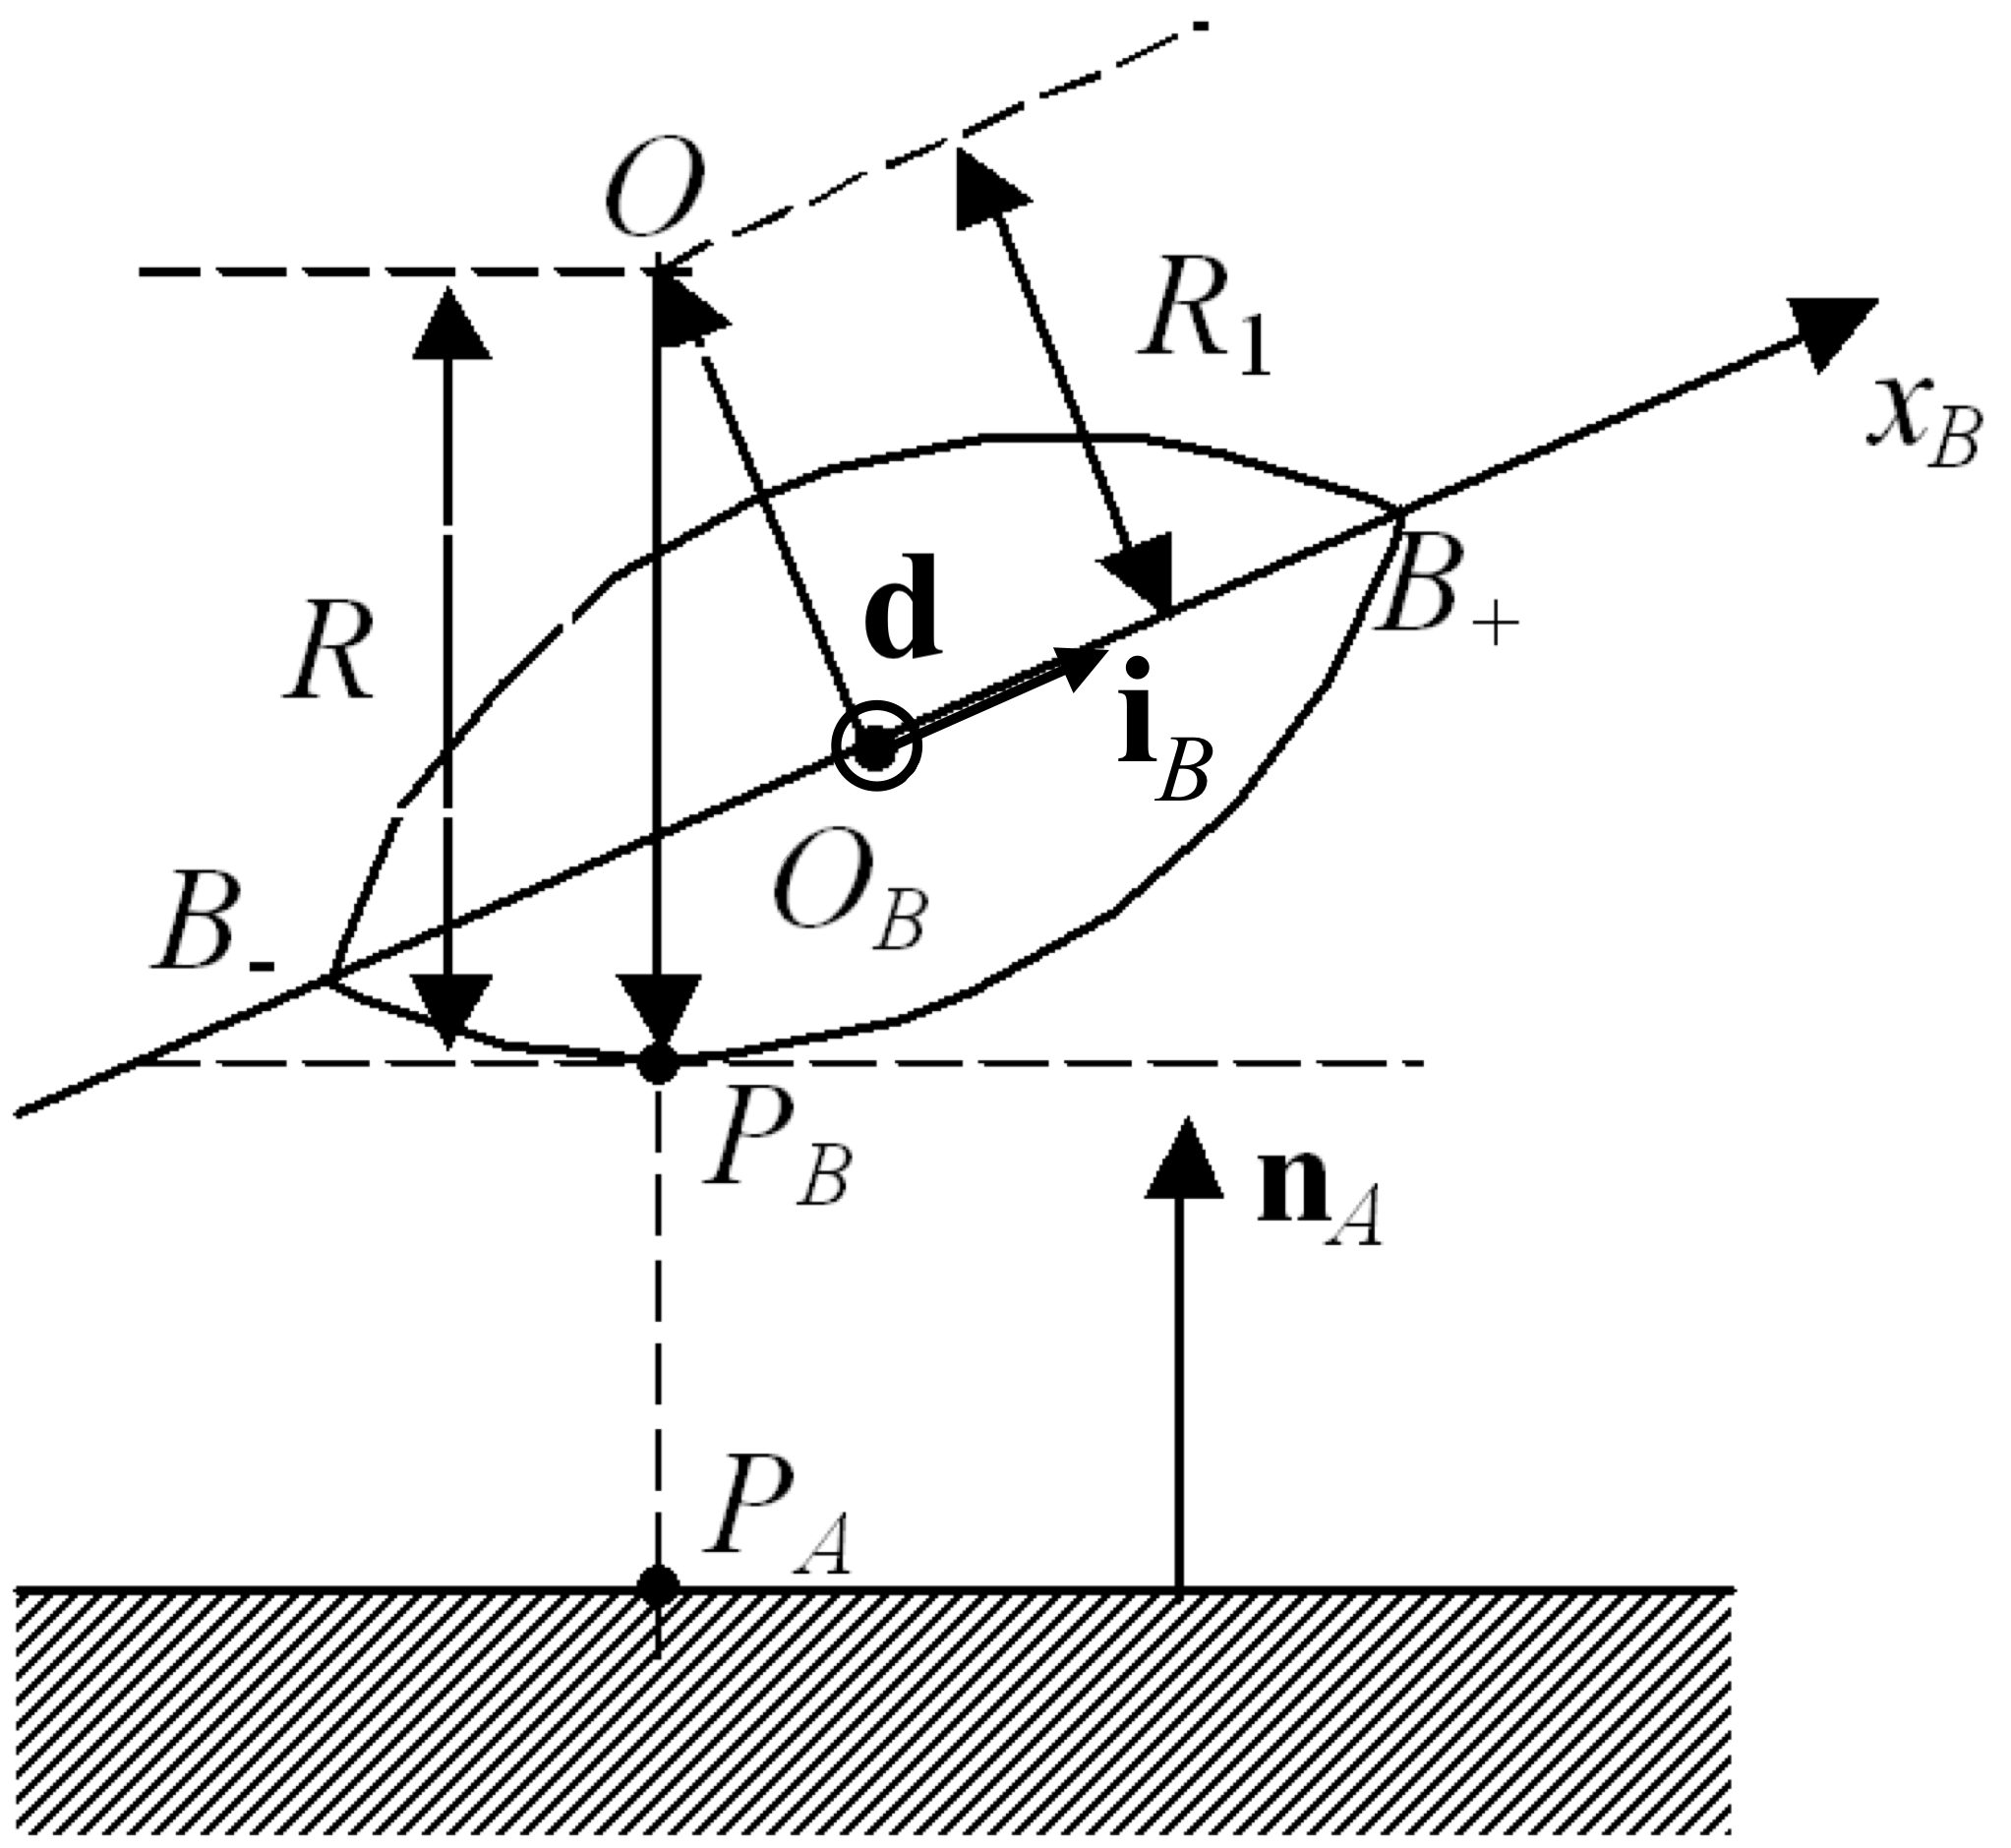
\includegraphics[width=8cm]{content/parts/3_friction/nd/RollerSection_d_ib.png}
    \asyinclude[width=12cm]{content/pic/asy/pic_roller_track.asy}
    \caption{Схема отслеживания контакта: вид сбоку отдельного ролика.}
    \label{ContactScheme}
\end{figure}

%Для вычисления положения точки $P_A$ нужно вторую координату 
%вектора ${\bf r}_{P_B}$ положить равной нулю
%\begin{equation}
%{\bf r}_{P_A}=\left( x_{P_B},0,z_{P_B}\right) ^T.
%\label{3_2_1}
%\end{equation}

% Все описанные выше вычисления справедливы только, если вектор $\vec{i}$ имеет направление, составляющее с вертикалью $\vec{\gamma}$ угол, ограниченный значениями $\pm\left(\ddfrac{\pi}{2} - \ddfrac{\pi}{n}\right)$. В противном случае следует положить $C = B_\pm$, где $B_{-}$ и $B_{+}$ -- левая и правая концевые точки ролика соответственно (см. рис.~\ref{ContactScheme}).

Контакт между роликом и опорной плоскостью имеет место, если и только если
\begin{equation}\label{cond:rol_vert}
    \left| \vec{i} \cdot \vec{\gamma} \right| \le \sin\ddfrac{\pi}{n},\quad Z_K < l
\end{equation}
где $Z_K$ -- расстояние от центра ролика до опорной плоскости.

Реализация контакта геометрически означает выполнение скалярного условия
\begin{equation}\label{cond:rol_zero}
    Z_C = 0,
\end{equation}
позволяющего, вместе с уравнениями динамики твердого тела, вычислить величину нормальной реакции $F_n$, приложенной в точке $C$. Отсутствие контакта доставляет выполнение альтернативного, также скалярного, условия равенства нормальной реакции нулю
$$
    F_n = 0.
$$

%\section{Отслеживание контакта в случае \textit{mecanum} колеса}
В разделе об \textbf{отслеживании контакта в случае \textit{mecanum} колеса} строится аналогичный алгоритм для нахождения координат точки контакта в случае, если ось ролика составляет ненулевой угол $\psi$ с плоскостью диска колеса.

%Обозначим угол наклона оси ролика к плоскости колеса $\psi$. В предыдущей конфигурации этот угол равен нулю. Расширим алгоритм отслеживания контакта, описанный выше для случая $\psi = 0$ на конфигурацию \textit{mecanum}, $\psi > 0$. В этом случае, в первую очередь, отметим отличия в геометрической форме роликов. Каждый ролик -- это твердое тело, ограниченное поверхностью вращения некоторой кривой вокруг его оси. В случае $\psi = 0$ эта кривая -- дуга окружности, но при $\psi > 0$, для того, чтобы проекция внежней границы колеса на его плоскость оставалась окружностью, форма роликов должна быть более сложной \cite{Gfrerrer2008}.
%
%\subsection{Неявный алгоритм отслеживания контакта}

\begin{figure}[H]
    \centering
    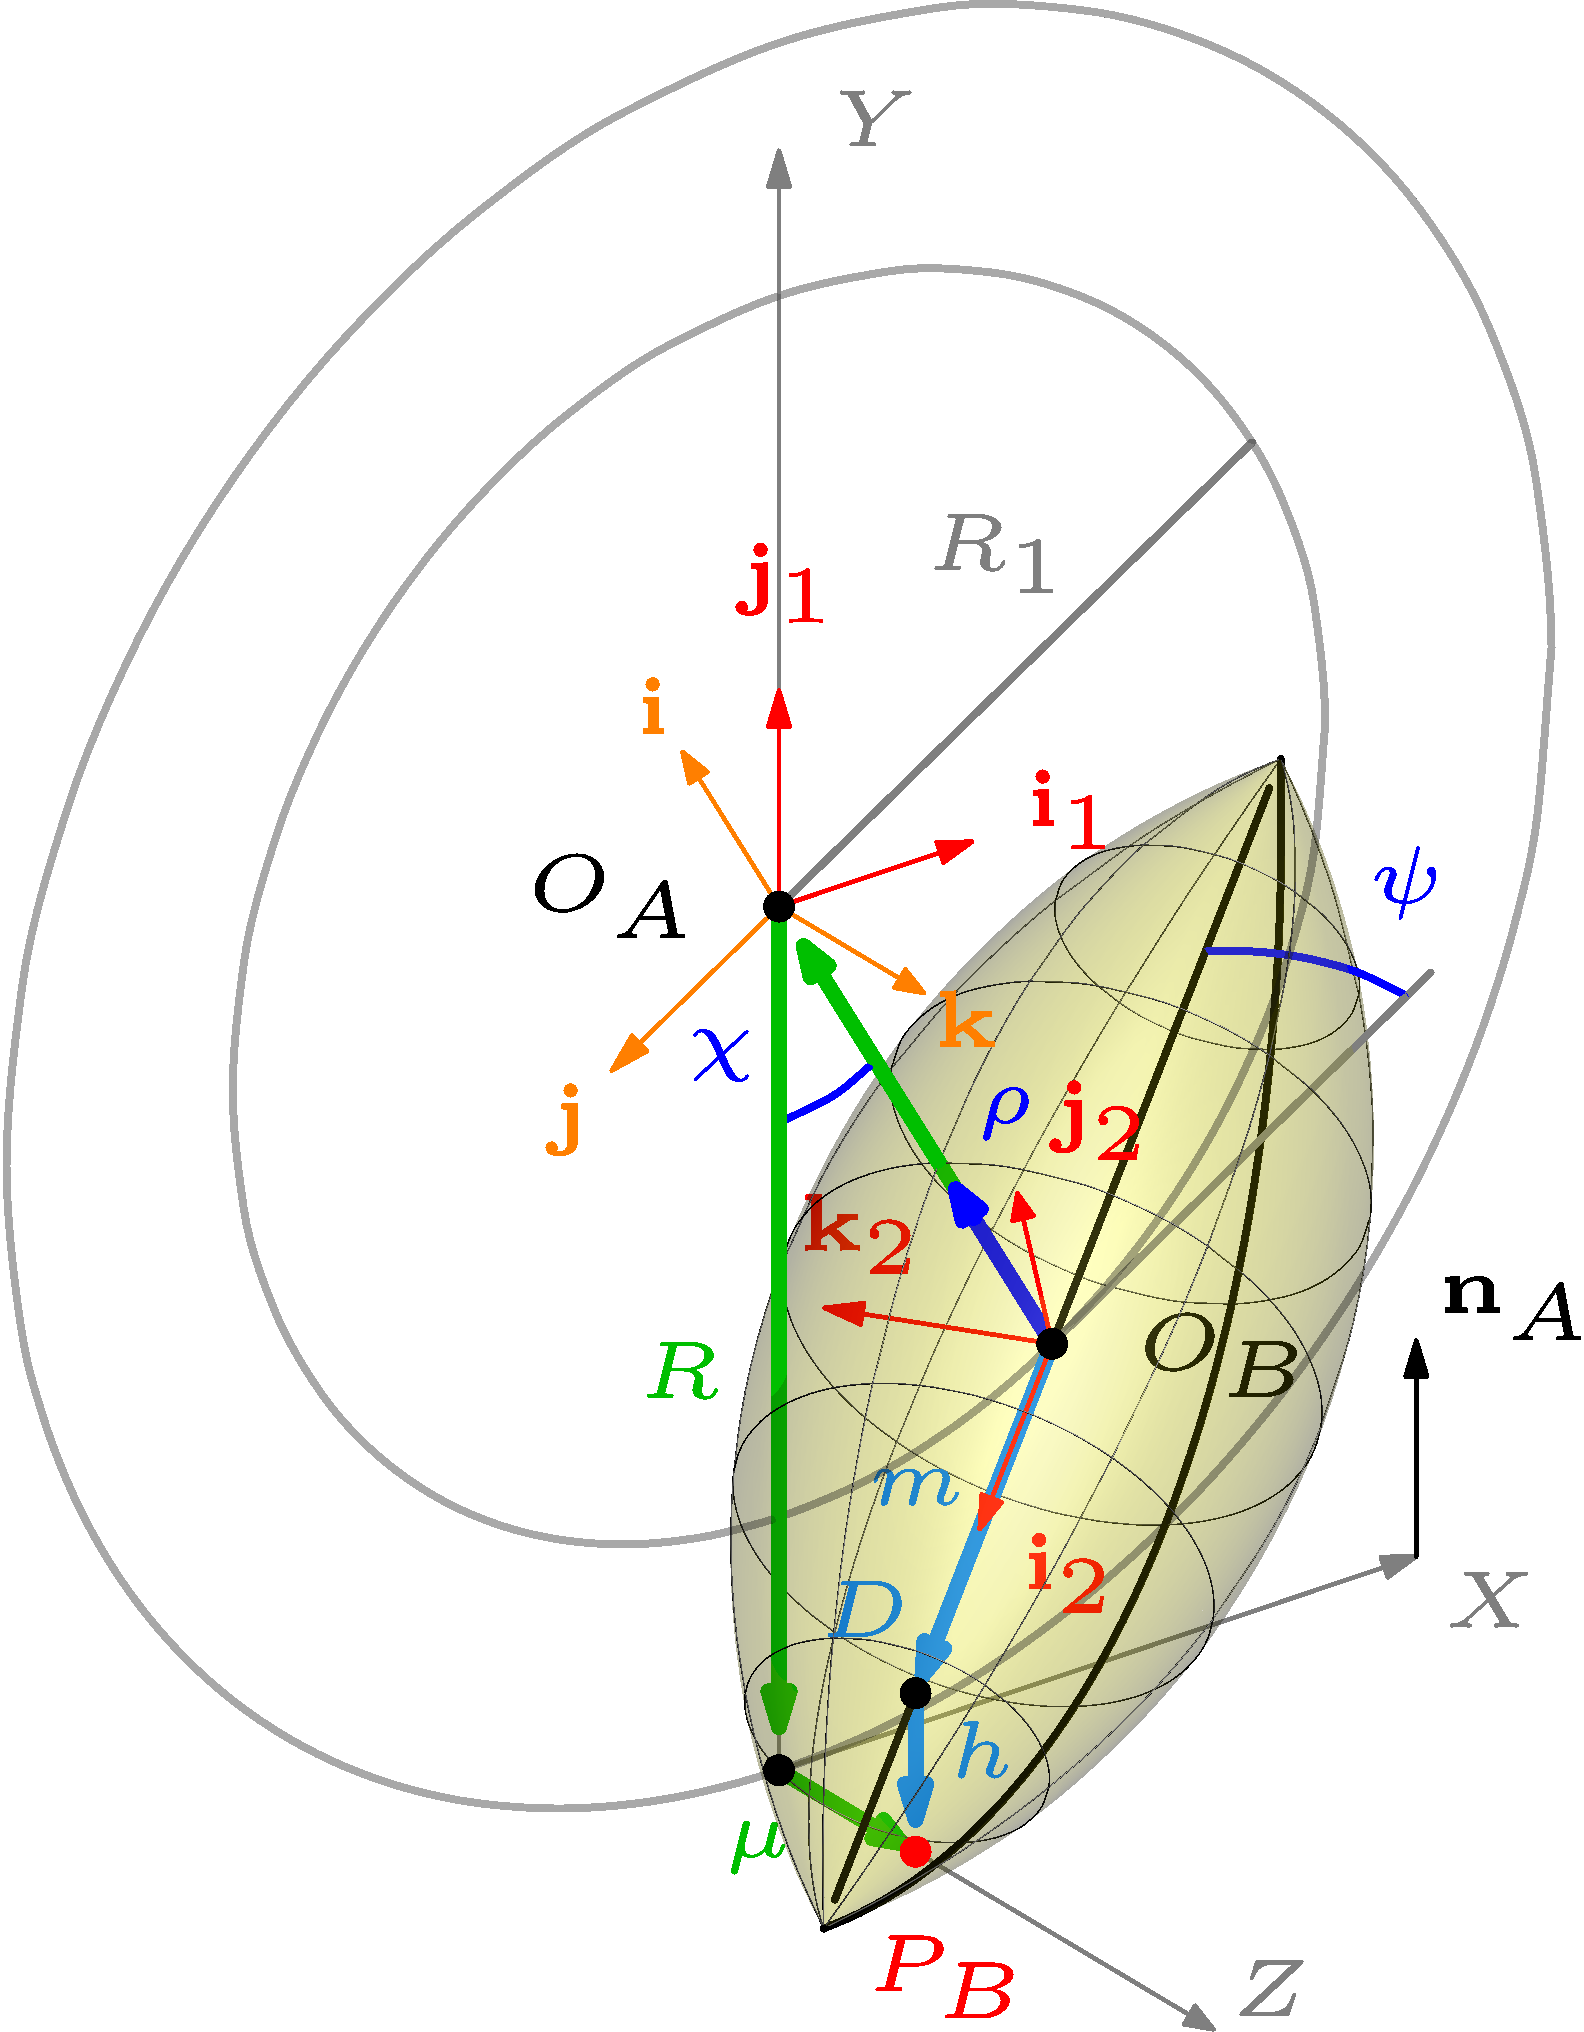
\includegraphics[width=0.5\textwidth]{./content/pic/asy/pic_mecanum.png}
    \caption{Отслеживание контакта для колеса \textit{mecanum}}
    \label{fig:mecanum}
\end{figure}

\textbf{Алгоритм отслеживания контакта} основан на наблюдении, что точка контакта находится всегда в пересечении вертикальной плоскости, содержащей ось колеса, и горизонтальной опорной плоскости. Координаты проекции центра колеса на опорную плоскость могут быть вычислены явно, и остается получить лишь расстояние $\mu$ от этой проекции до точки контакта вдоль отрезка линии пересечения плоскостей, соединяющего их, см. фиг.~\ref{fig:mecanum}.
Это делается из геометрических соображений и изложено в данном разделе.

% Величина $\mu$ может быть выражена из равенства
% $$
% {\bf r}_{P_B}={\bf r}_{O_B}+R_1\vecrho -R{\bf j}_1+\mu {\bf k}_1,
% $$
% после умножения его скалярно на ${\bf k}_2$:
% $$
% \mu =\left[R{\bf j}_1\cdot{\bf k}_2-R_1{\vecrho }\cdot {\bf k}_2\right] /
% {\bf k}_1\cdot{\bf k}_2,
% $$
% где компоненты вектора $\vecrho$ находятся с помощью кинематических соотношений
% $$
% \vecrho\cdot {\bf i}_2=0,\quad\vecrho\cdot {\bf k}_1=0.
% $$
% а компоненты векторов ${\bf i}_{(\cdot)},{\bf j}_{(\cdot)}$ определяются ориентацией тел в пространстве.

% При переходе колеса конструкции \textit{mecanum} с одного ролика на другой его след на плоскости терпит разрыв, поскольку точка контакта мгновенно переходит на противоположный <<борт>> колеса. Отмечается, что это обстоятельство, тем не менее, не препятствует эффективному численному решению.

В разделе \textbf{Моделирование трения в контакте} даются определения использованных моделей трения:
\begin{enumerate}
    \item {
        регуляризованное сухое трение
        $$
            \vec{F}_{\text{тр}} = -\mu N \vec{v}_{C}
                \left\{
                    \begin{array}{ll}
                        \ddfrac{1}{\delta}, \enspace |\vec{v}_{C}| < \delta \ll 1 \vspace{7pt}\\
                        \ddfrac{1}{|\vec{v}_{C}|}\enspace \text{иначе}
                    \end{array}
                \right.
        $$
    }
    \item {
        вязкое трение
        $$
            \vec{F}_{\text{тр}} = -\gamma\vec{v}_{C}
        $$
    }
\end{enumerate}

В разделе о \textbf{результатах численного моделирования} описаны результаты двух типов проведенных численных экспериментов.

Для сравнения модели экипажа на плоскости с сухим трением и безынерционной модели с неголономными связями проведены эксперименты для различных значений отношения $\massrel$ массы одного ролика к полной массе колеса. Показано, что с уменьшением этой величины, отличия угла курса $\theta$ экипажа и координат центра масс $x, y$ уменьшаются и становятся несущественными.
% , см. таблицу~\ref{tab:verif}.
Показано, что между роликами и опорной плоскостью может возникать скольжение при нахождении точки контакта в окрестности острого конца ролика, и скорость скольжения тем больше, чем тяжелее ролики.

Проведено качественное сравнение модели экипажа на плоскости с вязким трением и модели экипажа на абсолютно шероховатой плоскости, построенной в первых двух главах, на движении~3 из главы~2. Обнаружены динамические эффекты, аналогичные полученным в главе~2: характерный спиральный вид траектории центра масс, раскручивание роликов, возрастание угловой скорости платформы экипажа, одновременное с убыванием поступательной скорости её центра, последующее медленное убывание угловой скорости, убывание кинетической энергии экипажа. При расчетах коэффициент вязкого трения принимался достаточно большим: $10^{5}$. Такое значение позволило моделировать ударный характер переходных процессов при смене ролика в контакте. На гладких участках движения сходство с движением неголономной модели соответствует результату о близости движений неголономных систем и систем с вязким трением с достаточно большим коеффициентом.
% \cite{karapetyan1981negolonom}

% \begin{table}[ht]
%     \centering
%     \begin{tabular}{l|l|l}
%      & Движение $1$ & Движение $2$ \\ \hline
%     $\frac{m_{\text{рол}}}{m_{\text{к}}}$ &
%     $\Delta \theta$ &
%     $\max(|\Delta x|, |\Delta y|)$ \\ \hline
%     $10^{-1}$ & $\approx 1$       & $\approx 1$       \\
%     $10^{-2}$ & $\approx 10^{-1}$ & $\approx 0.5$     \\
%     $10^{-3}$ & $\approx 10^{-2}$ & $\approx 10^{-1}$ \\
%     $10^{-4}$ & $\approx 10^{-3}$ & $\approx 10^{-2}$ \\
%     $10^{-5}$ & $\approx 10^{-3}$ &                   \\
%     $10^{-6}$ & $\approx 10^{-4}$ & 
%     \end{tabular}
%     \caption{Сравнение моделей экипажа на плоскости с сухим трением и безынерционной модели с неголономными связями. Порядок различий в значениях угла курса платформы $\theta$ и координат центра масс $x, y$ экипажа при движениях $1$ и $2$ к моменту времени $t = 10$.}
%     \label{tab:verif}
% \end{table}